\documentclass[9pt]{beamer}
\usepackage{FiraSans}
\usetheme{metropolis}
\usepackage[utf8]{inputenc}
\usepackage{amsmath}
\usepackage{amsfonts}
\usepackage{amssymb}
\usepackage{multicol}
\usepackage{tikz}
\usepackage[T1]{fontenc} 
\usepackage[skins]{tcolorbox}
\author{Nicola Roman\`o - nicola.romano@ed.ac.uk}
\title{Unsupervised learning methods}
\setlength{\fboxsep}{0pt}
\setbeamertemplate{caption}{\raggedright\insertcaption\par}
\setbeamertemplate {footline}{\begin{scriptsize}\hfill\insertframenumber ~of \inserttotalframenumber\kern1em\vskip5pt\end{scriptsize}}

%\setbeamercovered{transparent} 
%\setbeamertemplate{navigation symbols}{} 

\titlegraphic{\centering 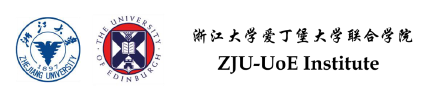
\includegraphics[scale=.5]{instituteLogo.png}}
%\institute{} 
\date{}
%\subject{} 

\begin{document}

\newtcolorbox{codebox}{enhanced,
				 top=2pt,
				 left=2pt,
				 right=2pt,
				 bottom=2pt,
				 boxrule=0pt,
				 leftrule=5pt,
				 sharp corners,				
				 colback=gray!20,
				 colframe=blue!60!black}

\begin{frame}
\titlepage
\end{frame}

\begin{frame}
{Learning objectives}
At the end of this lecture you should be able to:
\begin{itemize}
\item Explain the difference between supervised and unsupervised learning
\item Give examples of when these methods can be used
\item Explain the k-means and hierarchical clustering methods and discuss their advantages and disadvantages
\end{itemize}
\end{frame}

\begin{frame}
{Machine learning in biology}
\textbf{Some example problems we would like to be able to address}
\pause
\begin{enumerate}
\item We measure the amount of protein produced by a cell line in response to different intensities of a stimulus. We would like to predict the amount of protein after a stimulus of a different intensity.
\pause
\item We measure hormonal levels in healthy controls or patients with an illness. Given measures from a new individual, can we predict whether they are healthy or ill?
\pause
\item Given a set of photos of cells we want to divide depending on their shape.
\pause
\item Given measurements of expression of thousands of different genes from some tumour samples, we want to know whether there are specific classes of tumours, defined by a precise genetic signature.
\pause
\end{enumerate}
\textbf{How do we solve these problems?}
\end{frame}

\begin{frame}
{Problem 1}
We measure the amount of protein produced by a cell line in response to different intensities of a stimulus. We would like to predict the amount of protein after a stimulus of a different intensity.

\begin{overprint}
\onslide<1>\centering 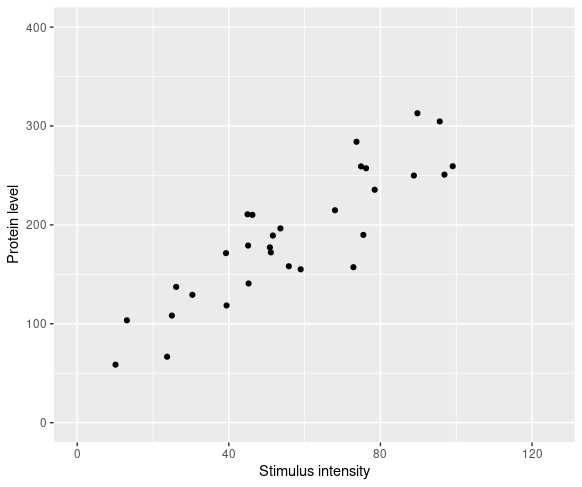
\includegraphics[width=0.5\textwidth]{Problem1.png}
\onslide<2>\centering 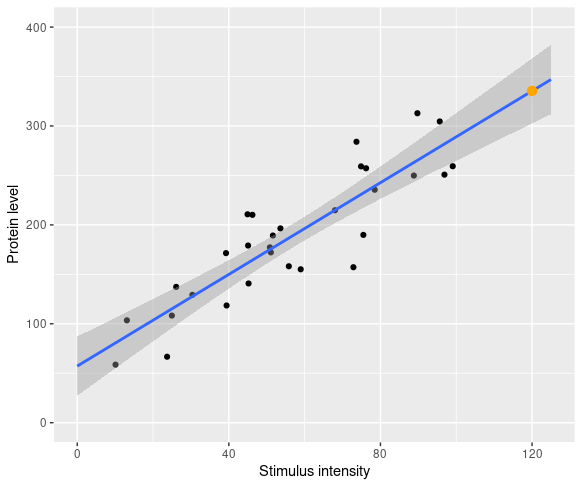
\includegraphics[width=0.5\textwidth]{Problem1b.png}
\end{overprint}
\onslide<2>\centering \textbf{Regression}

\begin{codebox}
\texttt{	lm(protein $\sim$ stimulus)}
\end{codebox}

\end{frame}

\begin{frame}
{Problem 2}
We measure hormonal levels in healthy controls or patients with an illness. Given measures from a new individual, can we predict whether they are healthy or ill?

\begin{overprint}
\onslide<1>\centering 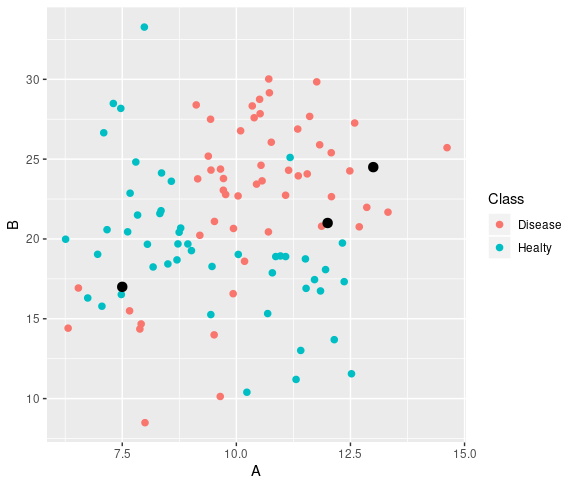
\includegraphics[width=0.55\textwidth]{Problem2.png}
\onslide<2>\centering {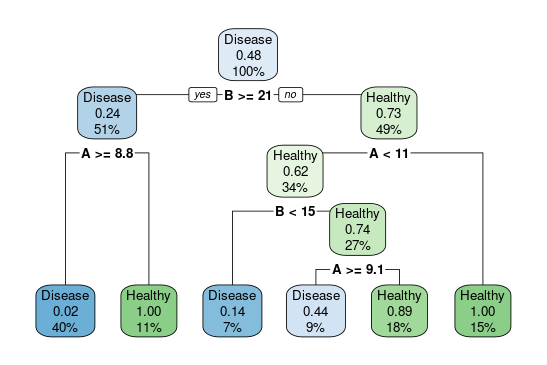
\includegraphics[height=120px]{Problem2-tree.png}~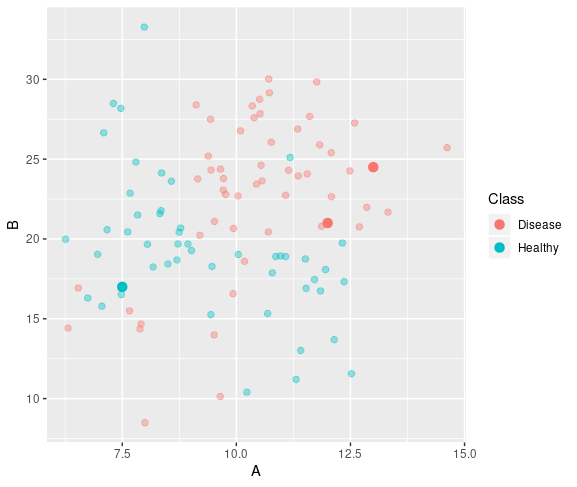
\includegraphics[height=120px]{Problem2-prediction.png}}
\end{overprint}
\onslide<2>\centering \textbf{Classification}

\begin{codebox}
\texttt{	rpart(Class $\sim$ A + B)}
\end{codebox}

\end{frame}

\begin{frame}
{Problem 3 and 4}

\begin{itemize}
\item Given a set of photos of cells we want to divide depending on their shape.\\
\centering 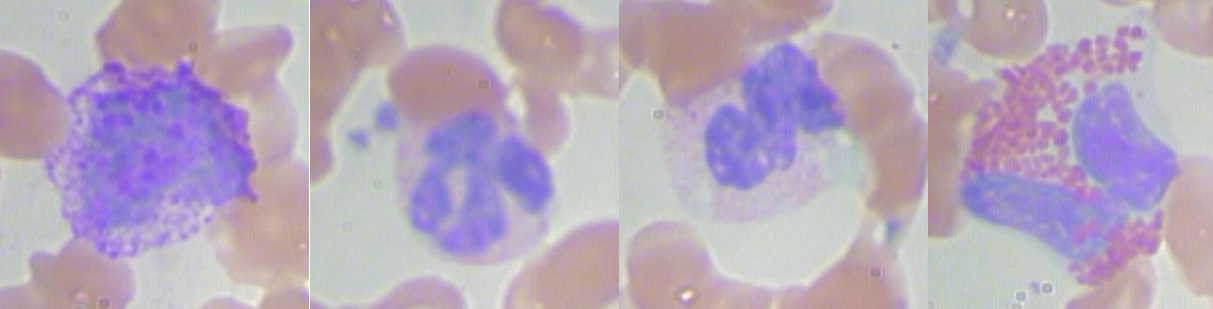
\includegraphics[width=0.4\textwidth]{celltypes.png}\\
\pause

\item Given measurements of expression of thousands of different genes from some tumour samples, we want to know whether there are specific classes of tumours, defined by a precise genetic signature.
\centering 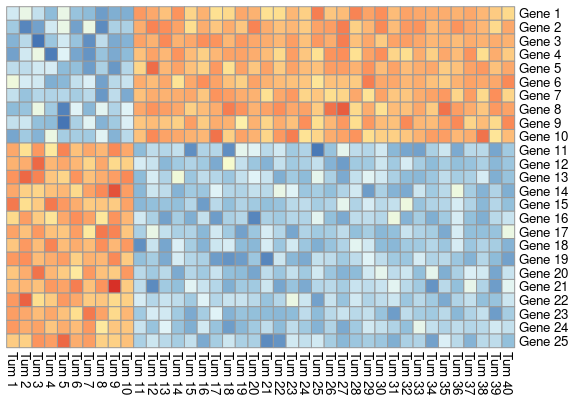
\includegraphics[width=0.5\textwidth]{heatmap.png}
\end{itemize}
\pause
\begin{center}
\textbf{How to do this?} We don't have information to train a model.
\end{center}
\end{frame}

\begin{frame}
{Supervised vs unsupervised learning}

Machine learning methods can be broadly divided into supervised and unsupervised.

\textbf{Supervised methods}
\begin{itemize}
\item We train a model using a training set with known labels
\item We test the accuracy of the model on a test set with known labels, but that we did not use for training.
\item We can use the model for prediction/classification.
\item Examples: binary trees, RandomForest, SVM, Neural Networks, ...
\end{itemize}
\pause
\textbf{Unsupervised methods}
\begin{itemize}
\item We have an unlabelled dataset. 
\item We use a model to find data patterns/groupings (\textbf{clustering}).
\item Examples: k-means, hierarchical clustering (this lecture), dimensionality reduction (next lecture)...
\end{itemize}
\end{frame}

\begin{frame}
{Clustering}
\textbf{Cluster analysis} or \textbf{clustering} is the task of grouping a set of objects in such a way that objects in the same group (called a cluster) are more similar (in some sense) to each other than to those in other groups (clusters). (\textit{Wikipedia})
\pause

\centering 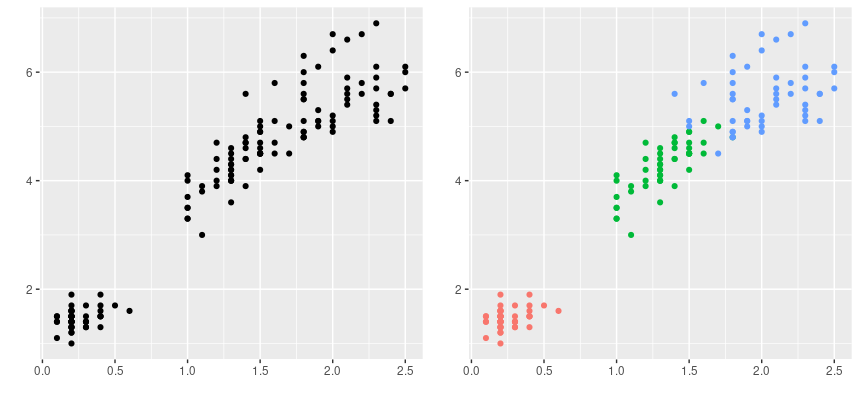
\includegraphics[width=0.8\textwidth]{clustering.png}\\

\pause
\textbf{The number of clusters in an unknown data set is not trivial to determine.}
\end{frame}

\begin{frame}
{The k-means algorithm}

\begin{itemize}
\item One of the simplest approaches to clustering
\item It's an iterative algorithm that divides the dataset in k clusters
\end{itemize}
\end{frame}

\begin{frame}
{k-means - Step 1}
\begin{itemize}
\item We select k random points as starting centers (called \textit{centroids})
\item We assign each point in the dataset to the closest centroid, thus defining k clusters
\end{itemize}

\begin{overprint}
\onslide<1>\centering 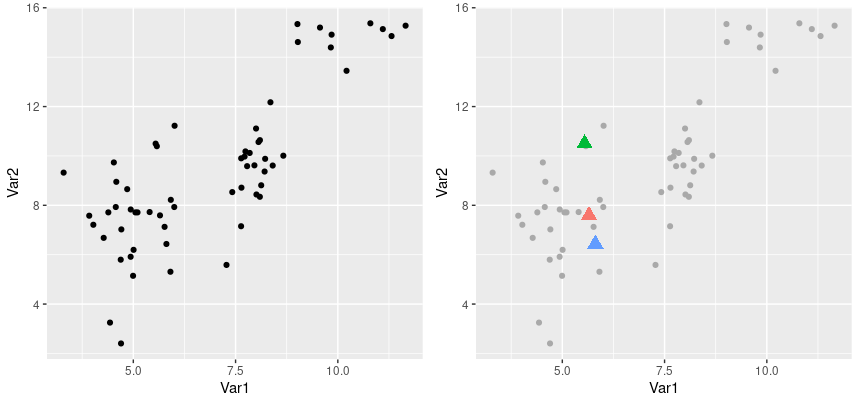
\includegraphics[height=150px]{kmeans-step1.png}
\onslide<2>\centering {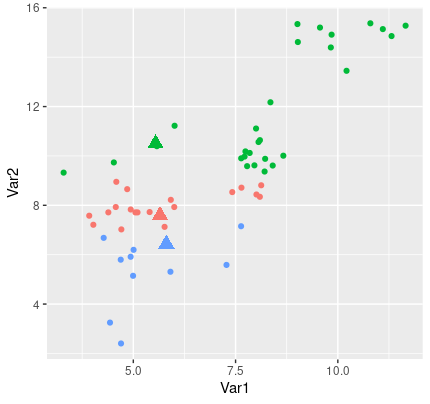
\includegraphics[height=150px]{kmeans-step2.png}}
\end{overprint}
\end{frame}

\begin{frame}
{k-means - Step 2}
\begin{itemize}
\item We move the centroids to the center of each cluster
\item We reassign cluster memberships and continue repeating until clusters don't change anymore or until we reach a certain number of iterations
\item Most often k-means converges after 10-20 iterations
\end{itemize}
\centering {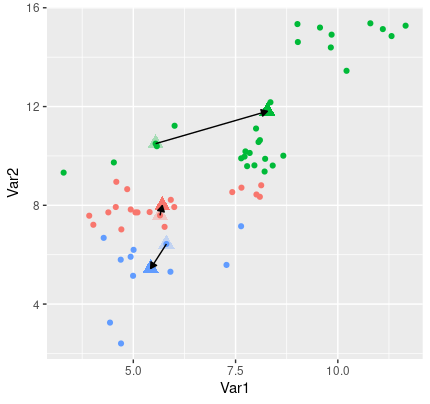
\includegraphics[height=150px]{kmeans-step3.png}}
\end{frame}

\begin{frame}
{k-means final clustering}
Our final result

\centering {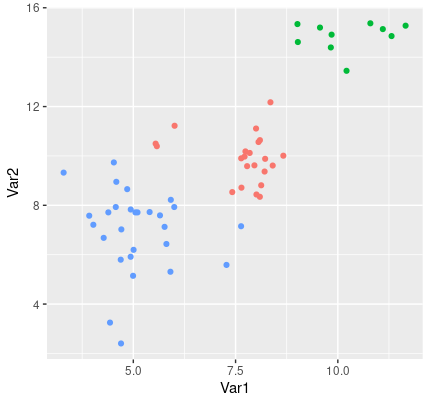
\includegraphics[height=150px]{kmeans-final.png}}
\end{frame}

\begin{frame}
{How to do k-means in R?}
It's really simple!

\begin{codebox}
\texttt{km <- kmeans(mydata, centers=3)}\\
\texttt{\# We can choose multiple sets of starting centroids}\\
\texttt{km <- kmeans(mydata, centers=3, nstart=50)}\\
\texttt{\# Clusters can be found in km\$cluster}
\end{codebox}

We will see some use of this in Workshop 7!
\end{frame}

\begin{frame}
{k-means pros and cons}
\textbf{Advantages}
\begin{itemize}
\item Generally fast
\item Computationally easy to implement
\end{itemize}

\textbf{Disadvantages}
\begin{itemize}
\item Results are heavily dependent on the random choice of centroids at the start
\item Need to specify the number of clusters in advance
\item Works better with equally sized clusters
\item Sensible to outliers

\end{itemize}
\end{frame}

\begin{frame}
{Determining number of clusters}
\begin{itemize}
\item Determining the number of clusters is difficult.
\item Depends on the question you are asking
\item There is no \textit{correct} solution
\pause
\item Empirical method - \textbf{elbow plot}
\begin{codebox}
\texttt{km\$tot.withinss / n.cluster}
\end{codebox}
\end{itemize}
\centering {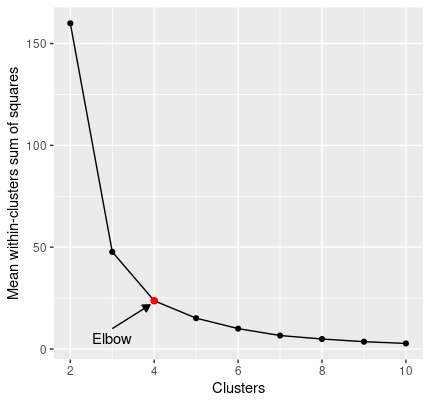
\includegraphics[height=150px]{elbowplot.png}}
\end{frame}

\begin{frame}
{Alternative strategy - hierarchical clustering}

\textbf{Hierarchical clustering} is a method of cluster analysis which seeks to build a hierarchy of clusters. (\textit{Wikipedia})

Two main strategies:
\begin{itemize}
\item Agglomerative or "bottom-up" hierarchical clustering initially creates one cluster per observation and then merge them depending on their similarity
\item Divisive or "top-down" hierarchical clustering puts all observations in one cluster then recursively splits the cluster.
\item Generates a \textit{dendrogram} (tree like plot)
\end{itemize}
\end{frame}

\begin{frame}
{Agglomerative hierarchical clustering}
\begin{itemize}
\item We start from n data points, each in a clusters
\item We define some distance metrics (see later)
\item We find the pair of points with the smaller distance
\item We start building our dendrogram
\end{itemize}

\begin{overprint}
\centering {\includegraphics<1>[height=120px]{hc1.png}
			\includegraphics<1>[height=120px]{hcdendro1.png}}
\centering {\includegraphics<2>[height=120px]{hc2.png}
			\includegraphics<2>[height=120px]{hcdendro2.png}}
\centering {\includegraphics<3>[height=120px]{hc3.png}
			\includegraphics<3>[height=120px]{hcdendro3.png}}
\centering {\includegraphics<4>[height=120px]{hc4.png}
			\includegraphics<4>[height=120px]{hcdendro4.png}}			
\end{overprint}
\end{frame}

\begin{frame}
{Agglomerative hierarchical clustering}
... and so on until every point has been clustered!
\centering 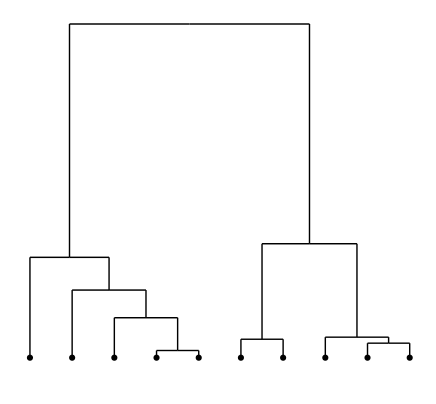
\includegraphics[height=120px]{finaldendro.png}
\pause
\begin{codebox}
\texttt{pt.dist  <- dist(hc, method = "euclidean")}\\
\texttt{hc <- hclust(pt.dist, method = "complete")}
\end{codebox}
\end{frame}

\begin{frame}
{How many clusters do we have?}
\centering 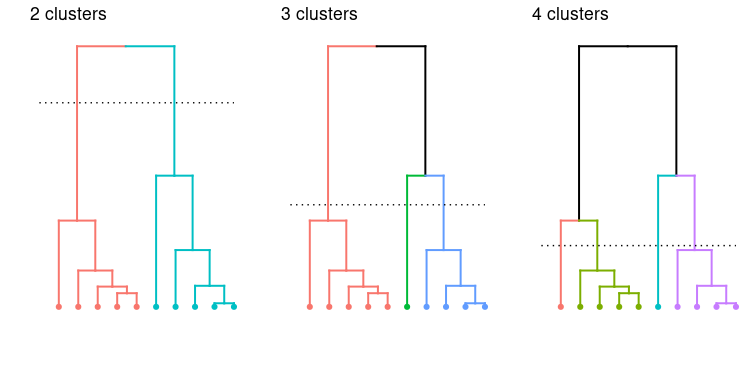
\includegraphics[height=140px]{hc5.png}
\end{frame}

\begin{frame}
{Distance methods}
\begin{codebox}
\texttt{pt.dist  <- dist(hc, \color{red}{\textbf{method = "euclidean"}})}
\end{codebox}

\begin{itemize}
\item The \texttt{method} parameter defines the metrics used for calculating the distance between data points
\item Several available (\texttt{"euclidean", "maximum", "manhattan", ...})
\pause
\item Given two data points A and B: $A(X1_A, X2_A, ..., Xn_A), B(X1_B, X2_B, ..., Xn_B)$\\
Euclidean distance $d = \sqrt{(X1_A-X1_B)^2+(X2_A-X2_B)^2+...+(Xn_A-Xn_B)^2}$
\pause
\item Maximum distance $d = max\{|X1_A-X1_B|, |X2_A-X2_B|, ..., |Xn_A-Xn_B|\}$
\pause
\item See \texttt{?dist} for full list and details
\end{itemize}
\end{frame}

\begin{frame}
{Linkages}
\begin{codebox}
\texttt{hc <- hclust(pt.dist, \color{red}{\textbf{method = "complete"}})}
\end{codebox}
\begin{itemize}
\item Similarly, the \texttt{method} parameter defines how the dendrogram is built
\item Common values are: \texttt{complete}, \texttt{average}, \texttt{ward.D2}
\item See \texttt{?hclust} for details

\end{itemize}
\end{frame}

\begin{frame}
{Summary}
\begin{itemize}
\item Statistical models and machine learning algorithms allow us to answer many biological questions
\item Choosing the right method to answer the right question is not easy
\item Clustering methods are becoming very important, especially when dealing with large dataset and/or data with high dimensionality (more on that in the next two data analysis lectures)
\item Many other approaches apart from those we saw today!
\end{itemize}
\end{frame}
\end{document}